% Options for packages loaded elsewhere
\PassOptionsToPackage{unicode}{hyperref}
\PassOptionsToPackage{hyphens}{url}
\PassOptionsToPackage{dvipsnames,svgnames,x11names}{xcolor}
%
\documentclass[
  letterpaper,
  DIV=11,
  numbers=noendperiod]{scrartcl}

\usepackage{amsmath,amssymb}
\usepackage{iftex}
\ifPDFTeX
  \usepackage[T1]{fontenc}
  \usepackage[utf8]{inputenc}
  \usepackage{textcomp} % provide euro and other symbols
\else % if luatex or xetex
  \usepackage{unicode-math}
  \defaultfontfeatures{Scale=MatchLowercase}
  \defaultfontfeatures[\rmfamily]{Ligatures=TeX,Scale=1}
\fi
\usepackage{lmodern}
\ifPDFTeX\else  
    % xetex/luatex font selection
\fi
% Use upquote if available, for straight quotes in verbatim environments
\IfFileExists{upquote.sty}{\usepackage{upquote}}{}
\IfFileExists{microtype.sty}{% use microtype if available
  \usepackage[]{microtype}
  \UseMicrotypeSet[protrusion]{basicmath} % disable protrusion for tt fonts
}{}
\makeatletter
\@ifundefined{KOMAClassName}{% if non-KOMA class
  \IfFileExists{parskip.sty}{%
    \usepackage{parskip}
  }{% else
    \setlength{\parindent}{0pt}
    \setlength{\parskip}{6pt plus 2pt minus 1pt}}
}{% if KOMA class
  \KOMAoptions{parskip=half}}
\makeatother
\usepackage{xcolor}
\setlength{\emergencystretch}{3em} % prevent overfull lines
\setcounter{secnumdepth}{-\maxdimen} % remove section numbering
% Make \paragraph and \subparagraph free-standing
\makeatletter
\ifx\paragraph\undefined\else
  \let\oldparagraph\paragraph
  \renewcommand{\paragraph}{
    \@ifstar
      \xxxParagraphStar
      \xxxParagraphNoStar
  }
  \newcommand{\xxxParagraphStar}[1]{\oldparagraph*{#1}\mbox{}}
  \newcommand{\xxxParagraphNoStar}[1]{\oldparagraph{#1}\mbox{}}
\fi
\ifx\subparagraph\undefined\else
  \let\oldsubparagraph\subparagraph
  \renewcommand{\subparagraph}{
    \@ifstar
      \xxxSubParagraphStar
      \xxxSubParagraphNoStar
  }
  \newcommand{\xxxSubParagraphStar}[1]{\oldsubparagraph*{#1}\mbox{}}
  \newcommand{\xxxSubParagraphNoStar}[1]{\oldsubparagraph{#1}\mbox{}}
\fi
\makeatother

\usepackage{color}
\usepackage{fancyvrb}
\newcommand{\VerbBar}{|}
\newcommand{\VERB}{\Verb[commandchars=\\\{\}]}
\DefineVerbatimEnvironment{Highlighting}{Verbatim}{commandchars=\\\{\}}
% Add ',fontsize=\small' for more characters per line
\usepackage{framed}
\definecolor{shadecolor}{RGB}{241,243,245}
\newenvironment{Shaded}{\begin{snugshade}}{\end{snugshade}}
\newcommand{\AlertTok}[1]{\textcolor[rgb]{0.68,0.00,0.00}{#1}}
\newcommand{\AnnotationTok}[1]{\textcolor[rgb]{0.37,0.37,0.37}{#1}}
\newcommand{\AttributeTok}[1]{\textcolor[rgb]{0.40,0.45,0.13}{#1}}
\newcommand{\BaseNTok}[1]{\textcolor[rgb]{0.68,0.00,0.00}{#1}}
\newcommand{\BuiltInTok}[1]{\textcolor[rgb]{0.00,0.23,0.31}{#1}}
\newcommand{\CharTok}[1]{\textcolor[rgb]{0.13,0.47,0.30}{#1}}
\newcommand{\CommentTok}[1]{\textcolor[rgb]{0.37,0.37,0.37}{#1}}
\newcommand{\CommentVarTok}[1]{\textcolor[rgb]{0.37,0.37,0.37}{\textit{#1}}}
\newcommand{\ConstantTok}[1]{\textcolor[rgb]{0.56,0.35,0.01}{#1}}
\newcommand{\ControlFlowTok}[1]{\textcolor[rgb]{0.00,0.23,0.31}{\textbf{#1}}}
\newcommand{\DataTypeTok}[1]{\textcolor[rgb]{0.68,0.00,0.00}{#1}}
\newcommand{\DecValTok}[1]{\textcolor[rgb]{0.68,0.00,0.00}{#1}}
\newcommand{\DocumentationTok}[1]{\textcolor[rgb]{0.37,0.37,0.37}{\textit{#1}}}
\newcommand{\ErrorTok}[1]{\textcolor[rgb]{0.68,0.00,0.00}{#1}}
\newcommand{\ExtensionTok}[1]{\textcolor[rgb]{0.00,0.23,0.31}{#1}}
\newcommand{\FloatTok}[1]{\textcolor[rgb]{0.68,0.00,0.00}{#1}}
\newcommand{\FunctionTok}[1]{\textcolor[rgb]{0.28,0.35,0.67}{#1}}
\newcommand{\ImportTok}[1]{\textcolor[rgb]{0.00,0.46,0.62}{#1}}
\newcommand{\InformationTok}[1]{\textcolor[rgb]{0.37,0.37,0.37}{#1}}
\newcommand{\KeywordTok}[1]{\textcolor[rgb]{0.00,0.23,0.31}{\textbf{#1}}}
\newcommand{\NormalTok}[1]{\textcolor[rgb]{0.00,0.23,0.31}{#1}}
\newcommand{\OperatorTok}[1]{\textcolor[rgb]{0.37,0.37,0.37}{#1}}
\newcommand{\OtherTok}[1]{\textcolor[rgb]{0.00,0.23,0.31}{#1}}
\newcommand{\PreprocessorTok}[1]{\textcolor[rgb]{0.68,0.00,0.00}{#1}}
\newcommand{\RegionMarkerTok}[1]{\textcolor[rgb]{0.00,0.23,0.31}{#1}}
\newcommand{\SpecialCharTok}[1]{\textcolor[rgb]{0.37,0.37,0.37}{#1}}
\newcommand{\SpecialStringTok}[1]{\textcolor[rgb]{0.13,0.47,0.30}{#1}}
\newcommand{\StringTok}[1]{\textcolor[rgb]{0.13,0.47,0.30}{#1}}
\newcommand{\VariableTok}[1]{\textcolor[rgb]{0.07,0.07,0.07}{#1}}
\newcommand{\VerbatimStringTok}[1]{\textcolor[rgb]{0.13,0.47,0.30}{#1}}
\newcommand{\WarningTok}[1]{\textcolor[rgb]{0.37,0.37,0.37}{\textit{#1}}}

\providecommand{\tightlist}{%
  \setlength{\itemsep}{0pt}\setlength{\parskip}{0pt}}\usepackage{longtable,booktabs,array}
\usepackage{calc} % for calculating minipage widths
% Correct order of tables after \paragraph or \subparagraph
\usepackage{etoolbox}
\makeatletter
\patchcmd\longtable{\par}{\if@noskipsec\mbox{}\fi\par}{}{}
\makeatother
% Allow footnotes in longtable head/foot
\IfFileExists{footnotehyper.sty}{\usepackage{footnotehyper}}{\usepackage{footnote}}
\makesavenoteenv{longtable}
\usepackage{graphicx}
\makeatletter
\def\maxwidth{\ifdim\Gin@nat@width>\linewidth\linewidth\else\Gin@nat@width\fi}
\def\maxheight{\ifdim\Gin@nat@height>\textheight\textheight\else\Gin@nat@height\fi}
\makeatother
% Scale images if necessary, so that they will not overflow the page
% margins by default, and it is still possible to overwrite the defaults
% using explicit options in \includegraphics[width, height, ...]{}
\setkeys{Gin}{width=\maxwidth,height=\maxheight,keepaspectratio}
% Set default figure placement to htbp
\makeatletter
\def\fps@figure{htbp}
\makeatother

\KOMAoption{captions}{tableheading}
\makeatletter
\@ifpackageloaded{caption}{}{\usepackage{caption}}
\AtBeginDocument{%
\ifdefined\contentsname
  \renewcommand*\contentsname{Table of contents}
\else
  \newcommand\contentsname{Table of contents}
\fi
\ifdefined\listfigurename
  \renewcommand*\listfigurename{List of Figures}
\else
  \newcommand\listfigurename{List of Figures}
\fi
\ifdefined\listtablename
  \renewcommand*\listtablename{List of Tables}
\else
  \newcommand\listtablename{List of Tables}
\fi
\ifdefined\figurename
  \renewcommand*\figurename{Figure}
\else
  \newcommand\figurename{Figure}
\fi
\ifdefined\tablename
  \renewcommand*\tablename{Table}
\else
  \newcommand\tablename{Table}
\fi
}
\@ifpackageloaded{float}{}{\usepackage{float}}
\floatstyle{ruled}
\@ifundefined{c@chapter}{\newfloat{codelisting}{h}{lop}}{\newfloat{codelisting}{h}{lop}[chapter]}
\floatname{codelisting}{Listing}
\newcommand*\listoflistings{\listof{codelisting}{List of Listings}}
\makeatother
\makeatletter
\makeatother
\makeatletter
\@ifpackageloaded{caption}{}{\usepackage{caption}}
\@ifpackageloaded{subcaption}{}{\usepackage{subcaption}}
\makeatother

\ifLuaTeX
  \usepackage{selnolig}  % disable illegal ligatures
\fi
\usepackage{bookmark}

\IfFileExists{xurl.sty}{\usepackage{xurl}}{} % add URL line breaks if available
\urlstyle{same} % disable monospaced font for URLs
\hypersetup{
  pdftitle={Class10: Structural Bioinformatics (pt1)},
  pdfauthor={Anyoleth Alarcon PID: A17347293},
  colorlinks=true,
  linkcolor={blue},
  filecolor={Maroon},
  citecolor={Blue},
  urlcolor={Blue},
  pdfcreator={LaTeX via pandoc}}


\title{Class10: Structural Bioinformatics (pt1)}
\author{Anyoleth Alarcon PID: A17347293}
\date{}

\begin{document}
\maketitle

\renewcommand*\contentsname{Table of contents}
{
\hypersetup{linkcolor=}
\setcounter{tocdepth}{3}
\tableofcontents
}

\subsection{The PDB Database}\label{the-pdb-database}

The main repository of biomolecular structure data is called the
\href{https://www.rcsb.org}{Protein Data Bank} (PDB for short). It is
the second oldest database (after GenBank).

What is currently in the PDB? We can access current composition stats
\href{https://www.rcsb.org/stats}{here}

\begin{Shaded}
\begin{Highlighting}[]
\NormalTok{stats }\OtherTok{\textless{}{-}} \FunctionTok{read.csv}\NormalTok{(}\StringTok{"Data Export Summary.csv"}\NormalTok{, }\AttributeTok{row.names =} \DecValTok{1}\NormalTok{)}
\FunctionTok{head}\NormalTok{(stats)}
\end{Highlighting}
\end{Shaded}

\begin{verbatim}
                          X.ray     EM    NMR Multiple.methods Neutron Other
Protein (only)          171,959 18,083 12,622              210      84    32
Protein/Oligosaccharide  10,018  2,968     34               10       2     0
Protein/NA                8,847  5,376    286                7       0     0
Nucleic acid (only)       2,947    185  1,535               14       3     1
Other                       170     10     33                0       0     0
Oligosaccharide (only)       11      0      6                1       0     4
                          Total
Protein (only)          202,990
Protein/Oligosaccharide  13,032
Protein/NA               14,516
Nucleic acid (only)       4,685
Other                       213
Oligosaccharide (only)       22
\end{verbatim}

\begin{quote}
Q1: What percentage of structures in the PDB are solved by X-Ray and
Electron Microscopy?
\end{quote}

\begin{Shaded}
\begin{Highlighting}[]
\NormalTok{x }\OtherTok{\textless{}{-}}\NormalTok{ stats}\SpecialCharTok{$}\NormalTok{X.ray}

\CommentTok{\# Substitute comma for nothing}
\NormalTok{y }\OtherTok{\textless{}{-}} \FunctionTok{gsub}\NormalTok{(}\StringTok{","}\NormalTok{, }\StringTok{""}\NormalTok{, x)}

\CommentTok{\# Convert to numeric}
\FunctionTok{sum}\NormalTok{(}\FunctionTok{as.numeric}\NormalTok{(y))}
\end{Highlighting}
\end{Shaded}

\begin{verbatim}
[1] 193952
\end{verbatim}

Turn this snippet into a function so I can use it any time I have this
comma problem (i.e.~the other columns of this `stats' table)

\begin{Shaded}
\begin{Highlighting}[]
\NormalTok{comma.sum }\OtherTok{\textless{}{-}} \ControlFlowTok{function}\NormalTok{(x) \{}
  \CommentTok{\# Substitute comma for nothing}
\NormalTok{  y }\OtherTok{\textless{}{-}} \FunctionTok{gsub}\NormalTok{(}\StringTok{","}\NormalTok{, }\StringTok{""}\NormalTok{, x)}

  \CommentTok{\# Convert to numeric and sum}
  \FunctionTok{return}\NormalTok{(}\FunctionTok{sum}\NormalTok{(}\FunctionTok{as.numeric}\NormalTok{(y)))}

\NormalTok{\}}
\end{Highlighting}
\end{Shaded}

\begin{Shaded}
\begin{Highlighting}[]
\NormalTok{xray.sum }\OtherTok{\textless{}{-}} \FunctionTok{comma.sum}\NormalTok{(stats}\SpecialCharTok{$}\NormalTok{X.ray)}
\NormalTok{em.sum }\OtherTok{\textless{}{-}} \FunctionTok{comma.sum}\NormalTok{(stats}\SpecialCharTok{$}\NormalTok{EM)}
\NormalTok{total.sum }\OtherTok{\textless{}{-}} \FunctionTok{comma.sum}\NormalTok{(stats}\SpecialCharTok{$}\NormalTok{Total)}
\end{Highlighting}
\end{Shaded}

\begin{Shaded}
\begin{Highlighting}[]
\NormalTok{xray.sum}\SpecialCharTok{/}\NormalTok{total.sum}\SpecialCharTok{*}\DecValTok{100}
\end{Highlighting}
\end{Shaded}

\begin{verbatim}
[1] 82.37223
\end{verbatim}

\begin{Shaded}
\begin{Highlighting}[]
\NormalTok{em.sum}\SpecialCharTok{/}\NormalTok{total.sum}\SpecialCharTok{*}\DecValTok{100}
\end{Highlighting}
\end{Shaded}

\begin{verbatim}
[1] 11.30648
\end{verbatim}

\begin{quote}
Q2: What proportion of structures in the PDB are protein?
\end{quote}

\begin{Shaded}
\begin{Highlighting}[]
\NormalTok{protein.sum }\OtherTok{\textless{}{-}} \FunctionTok{comma.sum}\NormalTok{(stats[}\DecValTok{1}\NormalTok{,}\DecValTok{7}\NormalTok{])}
\NormalTok{total.protein.sum }\OtherTok{\textless{}{-}} \FunctionTok{comma.sum}\NormalTok{(stats[,}\DecValTok{7}\NormalTok{])}
\NormalTok{protein.sum}\SpecialCharTok{/}\NormalTok{total.protein.sum}\SpecialCharTok{*}\DecValTok{100}
\end{Highlighting}
\end{Shaded}

\begin{verbatim}
[1] 86.2107
\end{verbatim}

\begin{quote}
Q3. Type HIV in the PDB website search box on the home page and
determine how many HIV-1 protease structures are in the current PDB?
\end{quote}

SKIPPED

\subsection{2. Visualizing with
Mol-star}\label{visualizing-with-mol-star}

Explore the HIV-1 protease structure with PDB code: \texttt{1HSG}
Mol-star homepage at: https://molstar.org/viewer/.

\begin{figure}[H]

{\centering 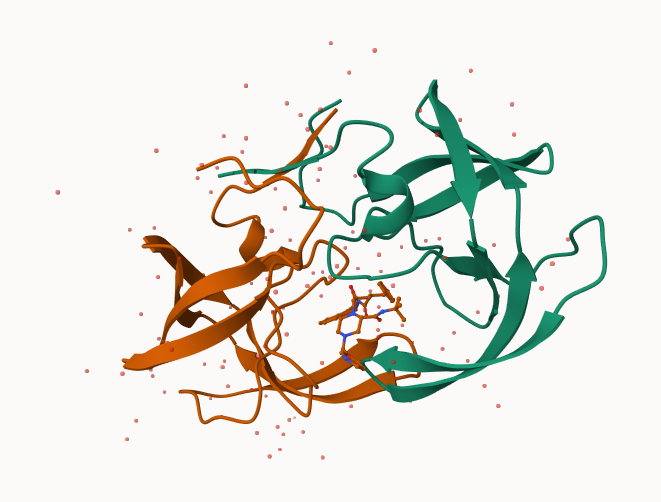
\includegraphics{1HSG.png}

}

\caption{Figure 1. A first view of HIV-Pr}

\end{figure}%%
\begin{figure}[H]

{\centering 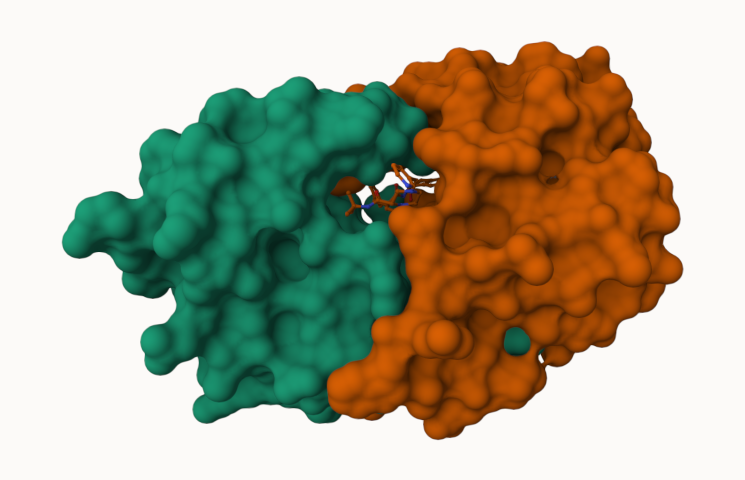
\includegraphics{1HSG1.png}

}

\caption{Figure 2. Molecular surface showing binding cavity}

\end{figure}%%
\begin{figure}[H]

{\centering 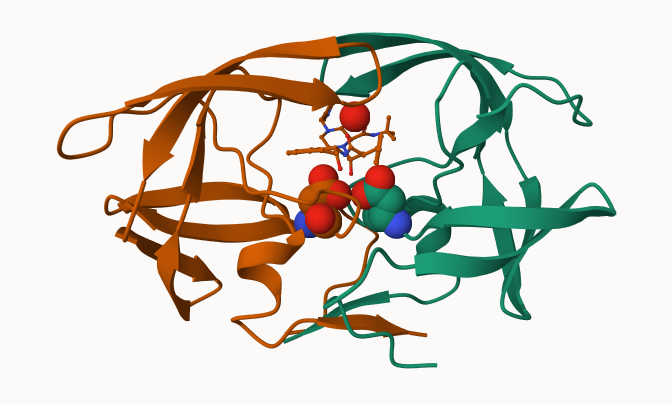
\includegraphics{1HSG2.png}

}

\caption{Figure 3. The catatilically important ASP amino acids and drug
interacting HOH 308 water molecule}

\end{figure}%

\subsection{3. Using the bio3d package in
R}\label{using-the-bio3d-package-in-r}

The Bio3D package is focused on structural bioinformatics analysis and
allows us to read and analyze PDB (and related) data.

\begin{Shaded}
\begin{Highlighting}[]
\FunctionTok{library}\NormalTok{(bio3d)}
\end{Highlighting}
\end{Shaded}

\begin{Shaded}
\begin{Highlighting}[]
\NormalTok{pdb }\OtherTok{\textless{}{-}} \FunctionTok{read.pdb}\NormalTok{(}\StringTok{"1hsg"}\NormalTok{)}
\end{Highlighting}
\end{Shaded}

\begin{verbatim}
  Note: Accessing on-line PDB file
\end{verbatim}

\begin{Shaded}
\begin{Highlighting}[]
\NormalTok{pdb}
\end{Highlighting}
\end{Shaded}

\begin{verbatim}

 Call:  read.pdb(file = "1hsg")

   Total Models#: 1
     Total Atoms#: 1686,  XYZs#: 5058  Chains#: 2  (values: A B)

     Protein Atoms#: 1514  (residues/Calpha atoms#: 198)
     Nucleic acid Atoms#: 0  (residues/phosphate atoms#: 0)

     Non-protein/nucleic Atoms#: 172  (residues: 128)
     Non-protein/nucleic resid values: [ HOH (127), MK1 (1) ]

   Protein sequence:
      PQITLWQRPLVTIKIGGQLKEALLDTGADDTVLEEMSLPGRWKPKMIGGIGGFIKVRQYD
      QILIEICGHKAIGTVLVGPTPVNIIGRNLLTQIGCTLNFPQITLWQRPLVTIKIGGQLKE
      ALLDTGADDTVLEEMSLPGRWKPKMIGGIGGFIKVRQYDQILIEICGHKAIGTVLVGPTP
      VNIIGRNLLTQIGCTLNF

+ attr: atom, xyz, seqres, helix, sheet,
        calpha, remark, call
\end{verbatim}

\begin{Shaded}
\begin{Highlighting}[]
\FunctionTok{attributes}\NormalTok{(pdb)}
\end{Highlighting}
\end{Shaded}

\begin{verbatim}
$names
[1] "atom"   "xyz"    "seqres" "helix"  "sheet"  "calpha" "remark" "call"  

$class
[1] "pdb" "sse"
\end{verbatim}

We can see atom data with \texttt{pdb\$atom}:

\begin{Shaded}
\begin{Highlighting}[]
\FunctionTok{head}\NormalTok{(pdb}\SpecialCharTok{$}\NormalTok{atom)}
\end{Highlighting}
\end{Shaded}

\begin{verbatim}
  type eleno elety  alt resid chain resno insert      x      y     z o     b
1 ATOM     1     N <NA>   PRO     A     1   <NA> 29.361 39.686 5.862 1 38.10
2 ATOM     2    CA <NA>   PRO     A     1   <NA> 30.307 38.663 5.319 1 40.62
3 ATOM     3     C <NA>   PRO     A     1   <NA> 29.760 38.071 4.022 1 42.64
4 ATOM     4     O <NA>   PRO     A     1   <NA> 28.600 38.302 3.676 1 43.40
5 ATOM     5    CB <NA>   PRO     A     1   <NA> 30.508 37.541 6.342 1 37.87
6 ATOM     6    CG <NA>   PRO     A     1   <NA> 29.296 37.591 7.162 1 38.40
  segid elesy charge
1  <NA>     N   <NA>
2  <NA>     C   <NA>
3  <NA>     C   <NA>
4  <NA>     O   <NA>
5  <NA>     C   <NA>
6  <NA>     C   <NA>
\end{verbatim}

\begin{Shaded}
\begin{Highlighting}[]
\FunctionTok{head}\NormalTok{(}\FunctionTok{pdbseq}\NormalTok{(pdb))}
\end{Highlighting}
\end{Shaded}

\begin{verbatim}
  1   2   3   4   5   6 
"P" "Q" "I" "T" "L" "W" 
\end{verbatim}

We can make quick 3D viz with the \texttt{view.pdb()} function.

\begin{Shaded}
\begin{Highlighting}[]
\FunctionTok{library}\NormalTok{(bio3dview)}
\FunctionTok{library}\NormalTok{(NGLVieweR)}

 \CommentTok{\# view.pdb(pdb, backgroundColor = "pink", colorScheme = "sse")}
\end{Highlighting}
\end{Shaded}

\begin{Shaded}
\begin{Highlighting}[]
\NormalTok{sel }\OtherTok{\textless{}{-}} \FunctionTok{atom.select}\NormalTok{(pdb, }\AttributeTok{resno=}\DecValTok{25}\NormalTok{)}

 \CommentTok{\# view.pdb(pdb, cols=c("green", "orange"),}
  \CommentTok{\#       highlight = sel,}
  \CommentTok{\#       highlight.style = "spacefill") |\textgreater{}}
 \CommentTok{\# setRock()}
\end{Highlighting}
\end{Shaded}

\subsection{Predicting functional motions of a single
structure}\label{predicting-functional-motions-of-a-single-structure}

We can finish off today with a bioinformatics prediction of the
functional motions of a protein.

We will run a Normal Mode Analysis (NMA)

\begin{Shaded}
\begin{Highlighting}[]
\NormalTok{adk }\OtherTok{\textless{}{-}} \FunctionTok{read.pdb}\NormalTok{(}\StringTok{"6s36"}\NormalTok{)}
\end{Highlighting}
\end{Shaded}

\begin{verbatim}
  Note: Accessing on-line PDB file
   PDB has ALT records, taking A only, rm.alt=TRUE
\end{verbatim}

\begin{Shaded}
\begin{Highlighting}[]
\NormalTok{adk}
\end{Highlighting}
\end{Shaded}

\begin{verbatim}

 Call:  read.pdb(file = "6s36")

   Total Models#: 1
     Total Atoms#: 1898,  XYZs#: 5694  Chains#: 1  (values: A)

     Protein Atoms#: 1654  (residues/Calpha atoms#: 214)
     Nucleic acid Atoms#: 0  (residues/phosphate atoms#: 0)

     Non-protein/nucleic Atoms#: 244  (residues: 244)
     Non-protein/nucleic resid values: [ CL (3), HOH (238), MG (2), NA (1) ]

   Protein sequence:
      MRIILLGAPGAGKGTQAQFIMEKYGIPQISTGDMLRAAVKSGSELGKQAKDIMDAGKLVT
      DELVIALVKERIAQEDCRNGFLLDGFPRTIPQADAMKEAGINVDYVLEFDVPDELIVDKI
      VGRRVHAPSGRVYHVKFNPPKVEGKDDVTGEELTTRKDDQEETVRKRLVEYHQMTAPLIG
      YYSKEAEAGNTKYAKVDGTKPVAEVRADLEKILG

+ attr: atom, xyz, seqres, helix, sheet,
        calpha, remark, call
\end{verbatim}

\begin{Shaded}
\begin{Highlighting}[]
\NormalTok{m }\OtherTok{\textless{}{-}} \FunctionTok{nma}\NormalTok{(adk)}
\end{Highlighting}
\end{Shaded}

\begin{verbatim}
 Building Hessian...        Done in 0.05 seconds.
 Diagonalizing Hessian...   Done in 0.5 seconds.
\end{verbatim}

\begin{Shaded}
\begin{Highlighting}[]
\FunctionTok{plot}\NormalTok{(m)}
\end{Highlighting}
\end{Shaded}

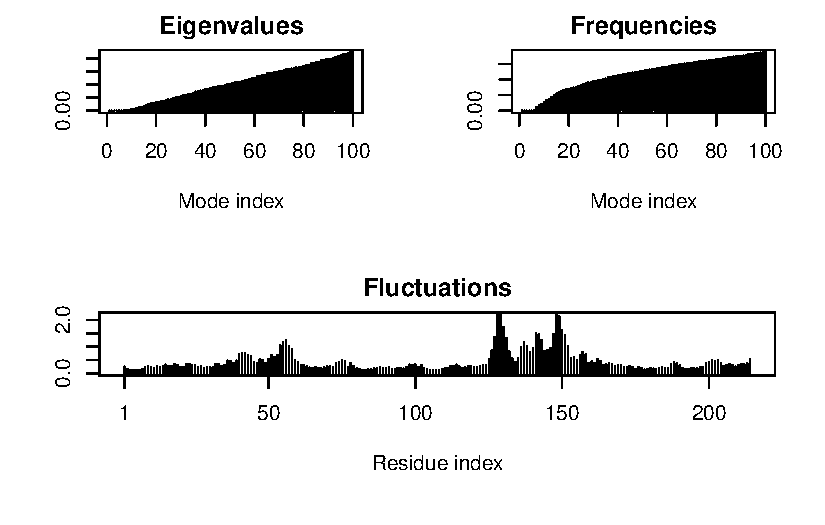
\includegraphics{Class10Structural_files/figure-pdf/unnamed-chunk-16-1.pdf}

\begin{Shaded}
\begin{Highlighting}[]
 \CommentTok{\# view.nma(m)}
\end{Highlighting}
\end{Shaded}

We can write-out a trajectory of the predicted dynamics and view this in
Mol-star.

\begin{Shaded}
\begin{Highlighting}[]
\FunctionTok{mktrj}\NormalTok{(m, }\AttributeTok{file=}\StringTok{"nma.pdb"}\NormalTok{)}
\end{Highlighting}
\end{Shaded}





\end{document}
